\begin{IEEEbiography} [{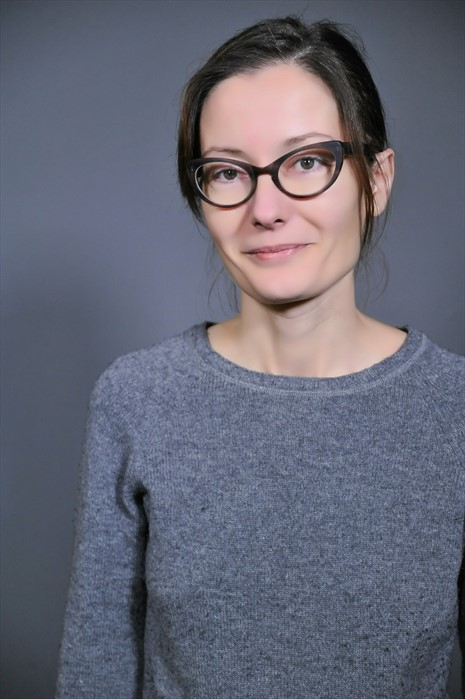
\includegraphics[width=1in,height=1.25in,clip,keepaspectratio]{images/Ronchieri}}]{Elisabetta Ronchieri}
is a Computer Science Engineer at INFN (Istituto Nazionale di Fisica Nucleare - National Institute of Nuclear Physics) CNAF. She holds a PhD in Automation, Robotics and Bioengineering from the University of Pisa. Her main area of interest include software engineering issues, such as software quality and software prediction model. She is also interested in (big and open) data analysis by using techniques coming from various theories, such as Machine Learning.
\end{IEEEbiography}

% if you will not have a photo at all:
\begin{IEEEbiography}[{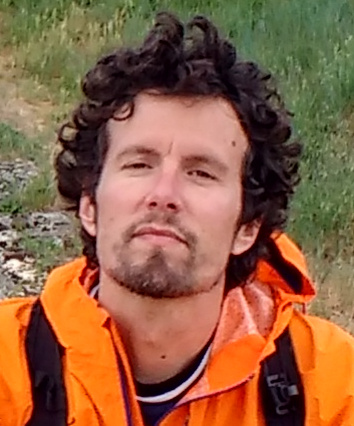
\includegraphics[width=1in,height=1.25in,clip,keepaspectratio]{images/pablo-orviz}}]{Pablo Orviz Fernandez}
is a computing researcher at CSIC (Consejo Superior de Investigaciones
Cientificas), holding an MSc in Scientific Computing from the University of
Cantabria. During the past years he has been devoted to software quality
assurance tasks within different European advanced computing research projects
such as INDIGO--DataCloud and EGI--Engage. Currently involved in EOSC--hub project
and participating in the software quality work packages of DEEP--HybridDataCloud
and eXtreme--DataCloud.
\end{IEEEbiography}

\begin{IEEEbiography}[{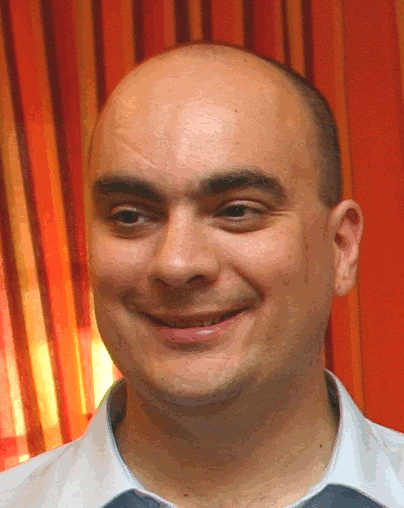
\includegraphics[width=1in,height=1.25in,clip,keepaspectratio]{images/mario-david}}]{Mario David}
is a research associate at LIP. He holds a PhD in Experimental Particle Physics from the University of Lisbon.
Member of DEEP--HybridDataCloud project as Work Package leader of Testbed and integration with EOSC services. Member of EOSC--hub project and
of the Portuguese National Computing Distributed Infrastructure.
He held a research associate position at Institut de Physique du Globe de Paris (IPGP/CNRS) as Scientific Software Developer for the VERCE project, in particular in the data intensive use cases for seismology.
He was been actively involved in the Validation, Quality Assurance and testing of middleware, in regional and global operations.
\end{IEEEbiography}

\begin{IEEEbiography}[{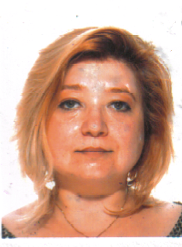
\includegraphics[width=1in,height=1.25in,clip,keepaspectratio]{images/cris_foto_good}}]{Doina Cristina Duma}
is the leader of the Distributed Systems group at the INFN National Center (CNAF), providing the core operational support for the INFN--wide Grid infrastructure and for the CNAF Cloud infrastructure. She has a long experience in managing distributed e--infrastructures, being involved since 2003 in major European projects such as DataGrid, EGEE (I, II, III), EGI--Inspire and EGI--Engage. She was the Release Manager of the EMI (European Middleware Initiative) and INDIGO - DataCloud European project project and having as main responsibilities to manage all release activities, including release planning, building, deploying, reporting, establishing and maintaining the overall release timeline and milestones.
\end{IEEEbiography}

\begin{IEEEbiography}[{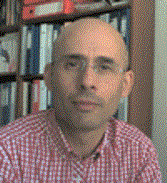
\includegraphics[width=1in,height=1.25in,clip,keepaspectratio]{images/jorge-gomes}}]{Jorge Gomes}
is a computing researcher at LIP. He worked in the development of advanced data acquisition systems at CERN, and participated in pioneering projects in the domain of digital satellite data communications, IP over ATM, and advanced videoconferencing over IP networks. Since 2001 he has participated in numerous projects regarding distributed computing, networks and security in Europe and Latin America. He is the head of the LIP Advanced Computing and Digital Infrastructures Group and technical coordinator of the Portuguese National Grid Infrastructure, representative of Portugal in the Council of the European Grid Infrastructure (EGI) and responsible for the Portuguese participation in IBERGRID, that joins Portuguese and Spanish distributed computing infrastructures.
\end{IEEEbiography}

\begin{IEEEbiography}[{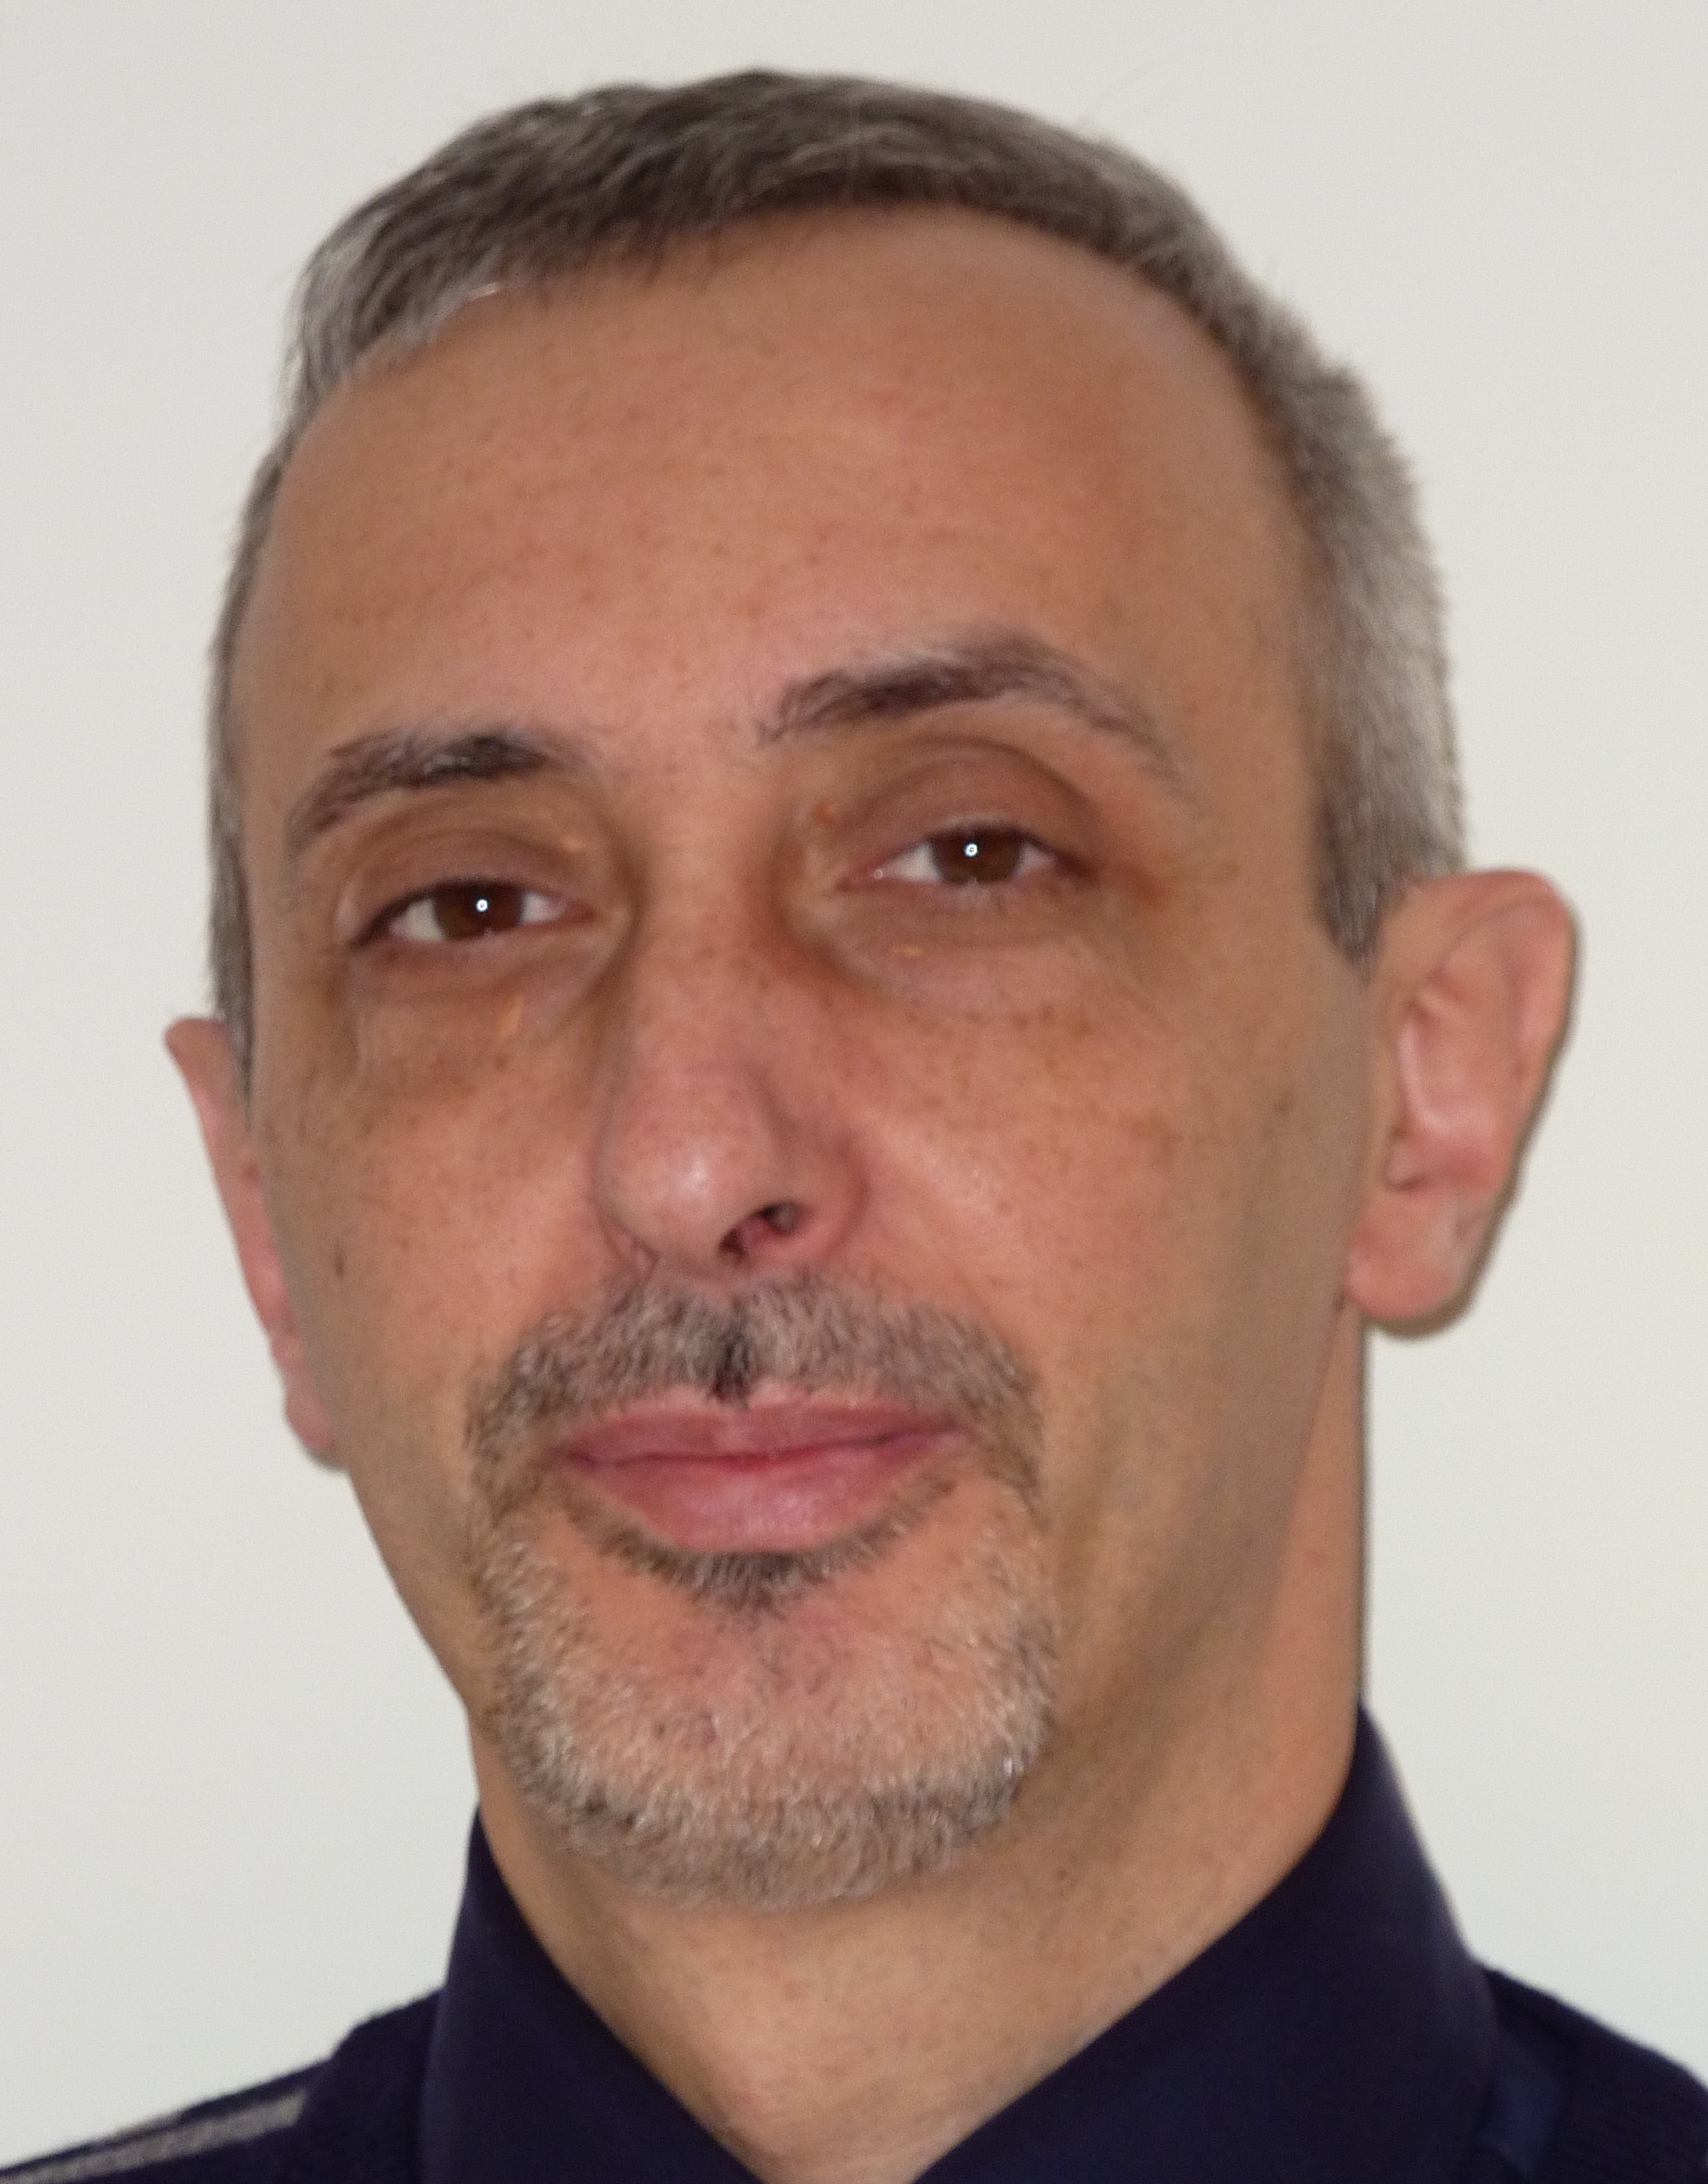
\includegraphics[width=1in,height=1.25in,clip,keepaspectratio]{images/DavideSalomoni}}]{Davide Salomoni}
is Director of Technology at the Italian National Institute for Nuclear Physics (INFN). He has 27 years of international experience in private and public environments related to distributed computing and communication technologies. He currently leads the Software Development and Distributed Systems department at CNAF, the INFN National Center dedicated to research and development on IT technologies, located in Bologna, Italy. He was Project Coordinator of INDIGO--DataCloud, a project funded by the EC Horizon2020, that developed innovative open source computing and storage solutions.
\end{IEEEbiography}

